% !TeX root=main.tex
% دستور زیر باید در اولین فصل شما باشد. آن را حذف نکنید!
\pagenumbering{arabic}

\chapter{مقدمه}
\thispagestyle{empty}
روش‌های سنتی یادگیری ماشین، معمولا روی مخزن‌های داده‌های ساکن و ایستا تمرکز کرده‌اند ولی توسعه فناوری، باعث شده است که داده‌های جریانی تولید شوند و راهی که مردم داده را ذخیره، و پردازش می‌کردند عوض شده است. امروزه بسیاری از سازمان‌ها، میزان زیادی از داده را با سرعت بالایی تولید می‌کند. به عنوان مثال، هر روز، گوگل بیشتر از سه و نیم میلیون جستجو را پاسخ می‌دهد\LTRfootnote{http://www.internetlivestats.com/google-search-statistics/}
، ماهواره‌های ناسا بیشتر از ۴ ترابایت عکس تولید می‌کنند\LTRfootnote{http://data.nasa.gov/about/}
 و فروشگاه والمارت بیشتر از ۲۰ میلیون تراکنش را ثبت می‌کند. مساله‌ای جدید تحقیقاتی داده‌کاوی و یادگیری ماشین این است: «چگونه ما می‌توانیم مجموعه‌ی داده‌ی نامحدودی که سریع تولید می‌شود و در طول زمان تغیری می‌کند را ضمن در نظر گرفتن محدودیت‌های زمانی و منابع محاسباتی مدل کنیم؟».

این مجموعه‌های داده بسیار بزرگ‌تر از آن هستند که روی حافظه‌ی اصلی جا شوند و باید روی حافظه‌های جانبی ذخیره بشوند. به علاوه، دسترسی تصادفی به این‌ داده‌ها که معمولا در روش‌های سنتی فرض می‌شد که امکان پذیر است، این‌جا بسار هزینه‌بر است. یک هدف کاوش داده‌های جریانی، ساختن یک فرایند یادگیری است که به صورت خطی با افزایش تعداد نمونه‌ها رشد کند. به هر حال از آنجایی که داده‌ها به شکل پیوسته در گذر هستند، مدلی که ما از روی داده‌های قدیمی می‌سازیم شاید به درد داده‌های جدید نخورد و باید اقر داده‌های منقضی‌شده از بین برود. این که مدل را با داده‌های جدید دوباره آموزش دهیم نیز فکری ناکارآمد و ناکافی است پس یک هدف کاوش داده‌های جریانی می‌تواند این باشد که چطور مدل را به صورت افزایشی با دیدن نمونه‌های جدید بروز رسانی کنیم.

\begin{table}
  \caption{مقایسه بین روش‌های یادگیری سنتی و روش‌های یادگیری در محیط داده‌های جریانی}
  \label{tbl:bound}
  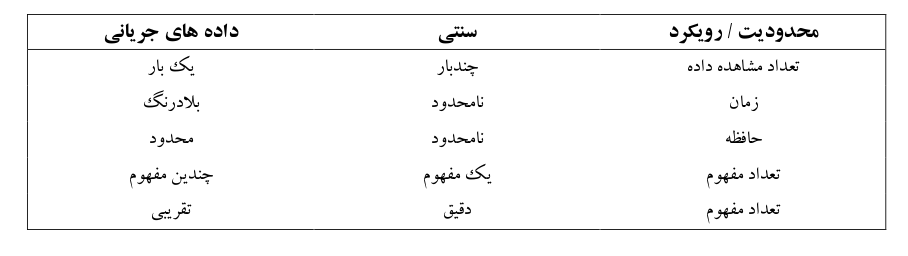
\includegraphics[width=\linewidth]{bound}
\end{table}


داده‌های جریانی با حجم نامتناهی، با اهمیت بودن ترتیب و زمان وقوع و تغییرات پویا شناخه می‌شوند. مثلا گوگل، میلیون‌های جستجو را روزانه پردازش می‌کند که هر کدامشان در یک زمان مشخص انجام شده‌اند و این جستجوها در طول زمان و براساس موضوعات داغ روز تغییر می‌کنند. جدول
\ref{tbl:bound}
تفاوت ویژگی‌های بین الگوریتم‌های داده‌های جریانی و الگوریتم‌های سنتی را نشان می‌دهد. به عبارت دیگر، اگر بخواهیم محدودیت‌های الگوریتم‌ها در فضای داده‌های جریانی را برشمریم باید از چهار محدودیت نام ببریم:


\begin{itemize}
\item یک‌بار مشاهده داده:\LTRfootnote{Single-pass } بر خلاف روش‌های یادگیری سنتی که می‌توانستند مجموعه‌‌ی داده را مکررا چند بار پیمایش کنند. الگوریتم‌ها در داده‌های جریانی فقط یک‌بار می‌توانند داده را مشاهده کنند و برگشت به عقبی وجود ندارد. دلیل این موضوع هم آن است که خواندن/نوشتن روی حافظه‌های جانبی بسیار هزینه‌بر تز از حافظه اصلی است. این محدودیت زیادی است و اگر به الگوریتم‌ها اجازه دهیم به جای یک داده چند داده را ببینند و اجازه داشته باشیند که چند نمونه به شکل کوتاه مدت ذخیره کنند اوضاع کمی بهتر می‌شود. به عنوان مثال یک الگوریتم می‌تواند یک دسته از نمونه‌ها را برای پردازش‌های داخلی ذخیره کند اما در نهایت باید با گرفتن یک دسته جدید از داده، داده‌های گذشته را پاک کند. 
\item پاسخ بلادرنگ:\LTRfootnote{Real-time Response} بسیاری از کاربردهای داده‌های جریانی نظیر پیش‌بینی بازار بورس، به پاسخ بلادرنگ نیاز دارند. میزان زمان مورد نیاز برای پردازش داده‌های و رسیدن به تصمیم باید کم باشد.
\item محدودیت حافظه: حجم‌ داده‌ای که می‌رسد خیلی بزرگ است و حتی ممکن است نامحدود باشد و ما می‌توانیم تنها تعداد کمی یا خلاصه‌ای از داده‌های جریانی را ذخیره‌ کنیم و ممکن است دیگر به اصل داده دسترسی نداشته باشیم. البته روش‌های تحمینی می‌توانند قابل قبول باشند.
\item تشخیص رانش‌ مفهوم: رانش‌ مفهوم زمانی است که الگوها(یا توزیع داده) در طی زمان تغییر پیدا می‌کند.
\end{itemize}

حال اگر منبع تولید جریان داده، منبعی باشد که متن تولید می‌کند مساله از جهاتی بغرنج‌تر می‌شود. پردازش و مدل‌کردن داده‌های متنی به دلیل غیر ساختیافته‌ بودن
\LTRfootnote{Unstructured}
، خطاهای سطح بالا
\LTRfootnote{High Level of Noise}
و وجود در فرمت‌های گوناگون بسیار پیچیده‌تر از سایر داده‌هاست. نفرین ابعاد
\LTRfootnote{Curse of Domensionality}
یکی از معضلات کار با داده‌های متنی است. در برخی از کاربردها، تعداد ویژگی‌هایی که از یک متن استخراج می‌شود چیزی بیش‌تر از دویست‌هزار ویژگی است. بنابراین لازم است که الگوریتم‌هایی در برابر داده‌های جریانی متنی به کار گرفته شوند که قابلیت سازگاری با این تعداد بسیار زیاد ویژگی را داشته باشند و یا این که با روش‌هایی نظیر پیش‌پردازش، انتخاب ویژگی و یا کاهش ابعاد، این داده‌ها را طوری به ورودی الگوریتم‌ها داد که محدودیت‌های زمانی و حافظه‌ای رعایت شود.
مضاف بر همه‌ی این مشکلات، در داده‌های متنی تعداد بسیار بیشتری از رویداد‌های تعجب‌آور و تغییر موضوعات شگفت‌انگیز مشاهده می‌شود. این موضوع باعث می‌شود که کاوش و یادگیری در داده‌های متنی یک وظیفه دلهره‌آور باشد. 








در این فصل به معرفی فضای کار در الگوریتم‌های یادگیری برای داده‌های جریانی پرداختیم، به علاوه مشکلات پیش‌رو زمانی که منبع داده‌ی ما یک منبع تولید کننده متن باشد را معرفی کردیم. در فصل‌ ۲ ابتدا به مرور ادبیات یادگیری در داده‌های جریانی خواهیم پرداخت و مفاهیمی نظیر منبع داده‌، مفهوم و رانش‌مفهوم را به شکل ریاضی تعریف می‌کنیم و سپس رویکردهای مختلف در برابر داده‌های جریانی را معرفی می‌کنیم. در این فصل علاوه بر ارایه تعاریف اولیه، مروری بر نرم‌افزارهای داده‌کاوی و یادگیری در فضای جریانی خواهیم داشت و مخزن‌های داده‌ی دردسترس را جهت تحقیقات و آزمایش‌های آتی معرفی خواهیم کرد. در فصل ۳ به معرفی الگوریتم‌های یادگیری ماشین در فضای داده های جریانی خواهیم پرداخت. این الگوریتم‌ها عموما نسخه‌های توسعه‌یافته از الگوریتم‌های سنتی یادگیری ماشین‌ هستند و با چالش‌ها و محدودیت‌های داده‌های جریانی سازگار شده‌اند. به طور کلی در این فصل الگوریتم‌هایی را معرفی خواهیم کرد که تغییر یافته الگوریتم‌های سنتی درخت تصمیم، یادگیرنده‌های بیز، شبکه‌های عصبی، ماشین‌های بردار پشتیبان و مجمع‌های رده‌بندی هستند. نهایتا در فصل ۴ و پایانی این گزارش، ابتدا به جمع‌بندی روش‌های یادگیری ارایه‌شده و مقایسه و نمایش نسبت الگوریتم‌ها با پدران سنتیشان می‌پردازیم سپس مزایا و معایب هر کدام را مطرح می‌کنیم و مشخص خواهیم کرد که کدام روش‌ها می‌توانند برای منابع جریانی داده‌های متنی به کار گرفته شوند. در نهایت نیز به جمع‌بندی کار و معرفی تحقیقات آینده،‌ نظیر انتخاب پویای ویژگی برای داده‌های جریانی خواهیم پرداخت.
